\section{Workload Drift Does Not Imply Useful Fast Adaptation}
\label{sec:workload-drift}

\begin{figure}[t]
    \centering
    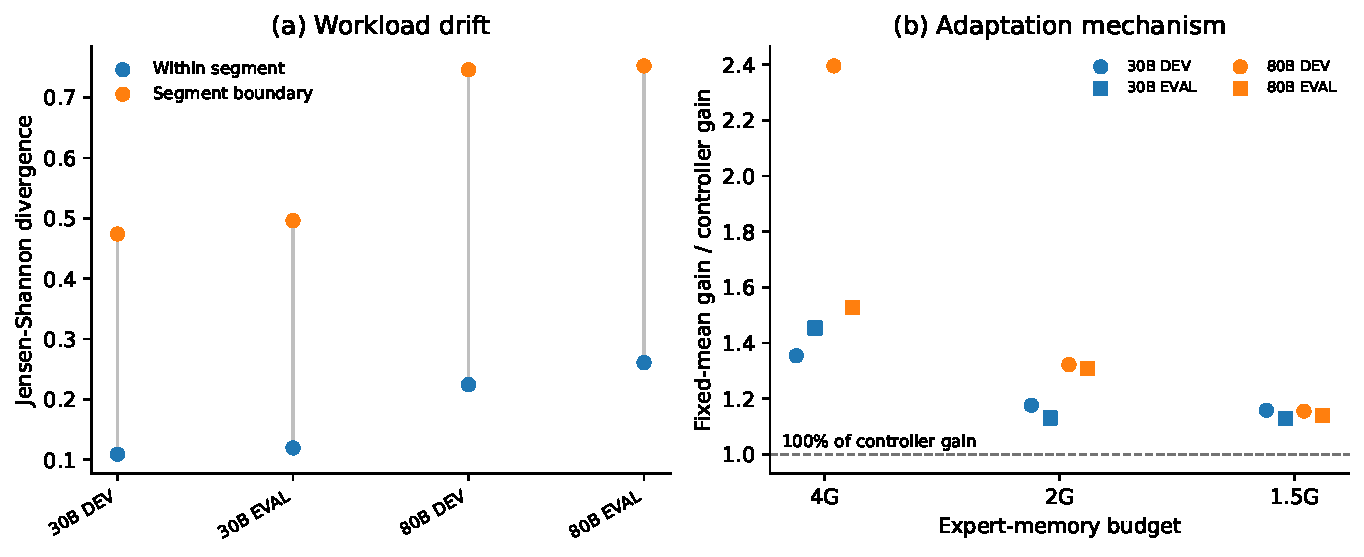
\includegraphics[width=\linewidth]{../experiments/EXP-023-workload-drift/figures/workload_drift_vs_adaptation.pdf}
    \caption{Workload drift does not imply useful fast adaptation. Panel (a) shows that Jensen--Shannon divergence between routing distributions is substantially larger across workload boundaries than within segments for both evaluated MoEs. Panel (b) compares the gain of a fixed allocation equal to the controller's mean allocation with the gain of the tested controller. The result confirms workload-dependent routing drift but falsifies the temporal mechanism of the current \texttt{adaptive-e64} controller; it does not establish that dynamic adaptation is ineffective in general.}
    \label{fig:workload-drift}
\end{figure}

The allocation results raise a natural temporal hypothesis: if workloads change, a controller that reacts to those changes may outperform a fixed layer partition. EXP-023 separates the two clauses of that hypothesis. The first clause---that routing distributions change at workload boundaries---is strongly supported descriptively. The second---that the current controller benefits from reacting rapidly to those changes---is falsified for \texttt{adaptive-e64}.

\subsection{Routing distributions move at workload boundaries}

The transition traces contain four segments with qualitatively different workloads. For each boundary and MoE layer, EXP-023 compares the last 64 counted decode steps of the outgoing segment with the first 64 of the incoming segment using Jensen--Shannon divergence. The reference is the JSD between adjacent non-overlapping 64-step windows within the corresponding segments.

\begin{table}[t]
    \centering
    \caption{Routing-distribution drift in the four transition traces. Ratios are medians of boundary JSD relative to the within-segment reference. This operationalization is retrospective and descriptive.}
    \label{tab:jsd-drift}
    \small
    \begin{tabular}{lrrr}
        \toprule
        Trace & Boundary JSD & Within JSD & Ratio \\
        \midrule
        30B DEV  & 0.4739 & 0.1091 & 3.810 \\
        30B EVAL & 0.4959 & 0.1196 & 4.022 \\
        80B DEV  & 0.7459 & 0.2246 & 3.381 \\
        80B EVAL & 0.7524 & 0.2608 & 2.839 \\
        \bottomrule
    \end{tabular}
\end{table}

Across all four traces, the median boundary divergence is 2.84--4.02 times the within-segment reference. Boundary JSD also exceeds the corresponding within-segment maximum in 96.5--100\% of layer-boundary rows. Workload transitions therefore induce large, repeatable changes in per-layer routing distributions.

This part of EXP-023 is deliberately not presented as a confirmatory hypothesis test: the JSD operationalization was fixed after the transition data already existed, and no $p$-value or success threshold was preregistered. Its role is descriptive characterization.

\subsection{The tested controller does not profit from fast reaction}

The temporal mechanism is tested independently of the JSD description. For each model, split, and budget, the analysis compares the controller's gain with a static allocation equal to the controller's \emph{mean} allocation over the trace. If the controller's advantage arose from timely movement of memory, averaging away that timing should remove a meaningful part of the gain.

It does not. The fixed mean allocation exceeds the controller's own gain in all 12 model/split/budget rows. The ratio of fixed-mean gain to controller gain ranges from 1.129 to 2.396. In addition, the reaction-lag cost relative to instantly switched segment allocations is negative in all 12 rows, ranging from $-1844$ to $-820$ misses. At individual boundaries, \texttt{adaptive-e64} has a lower signed 64-step departure from the new-segment steady state than the frozen split in only 11 of 36 comparisons; it is higher in 25 of 36.

\begin{proposition}[The temporal mechanism of \texttt{adaptive-e64} is falsified]
\label{prop:temporal-falsified}
For the four evaluated transition traces and three memory budgets, the observed gain of the current \texttt{adaptive-e64} controller cannot be attributed to beneficial rapid reaction to workload boundaries.
\end{proposition}

\begin{proof}
A timing-free comparator formed from the controller's own mean allocation matches or exceeds the controller gain in all 12 aggregate rows, while the measured reaction-lag comparison is unfavorable in all 12. Thus removing the temporal movement does not remove the gain; instead, the evidence attributes most or all of the benefit to the allocation partition itself rather than to fast transition response.
\end{proof}

The scope of Proposition~\ref{prop:temporal-falsified} is important. It does not imply that workloads are stationary, nor that dynamic adaptation is useless in general. The JSD measurements show the opposite: demand changes materially. The negative result applies to the current, untuned \texttt{adaptive-e64} temporal mechanism. A controller with better change detection, prediction, or faster actuation remains an open design direction.
